\documentclass[letterpaper,12pt]{article}
\usepackage[margin=.65in,top=.72in,bottom=.62in,headheight=16pt,headsep=15pt,footskip=19pt]{geometry}
\usepackage[T1]{fontenc}
\usepackage{lmodern,tikz,fancyhdr}\pdfmapfile{+lm.map}
\usetikzlibrary{arrows.meta,shapes.geometric}
\pagestyle{fancy}\fancyhf{}\renewcommand{\headrulewidth}{0pt}\renewcommand{\footrulewidth}{0pt}
\setlength{\parindent}{0pt}\setlength{\parskip}{0pt}
\fancyhead[L]{\small Week 44 / The bag that copies / K--1}
\fancyfoot[L]{\footnotesize Bellingham Math Circle / Week 44 / W44-k-1-v2}\fancyfoot[R]{\footnotesize\thepage}
\begin{document}
\noindent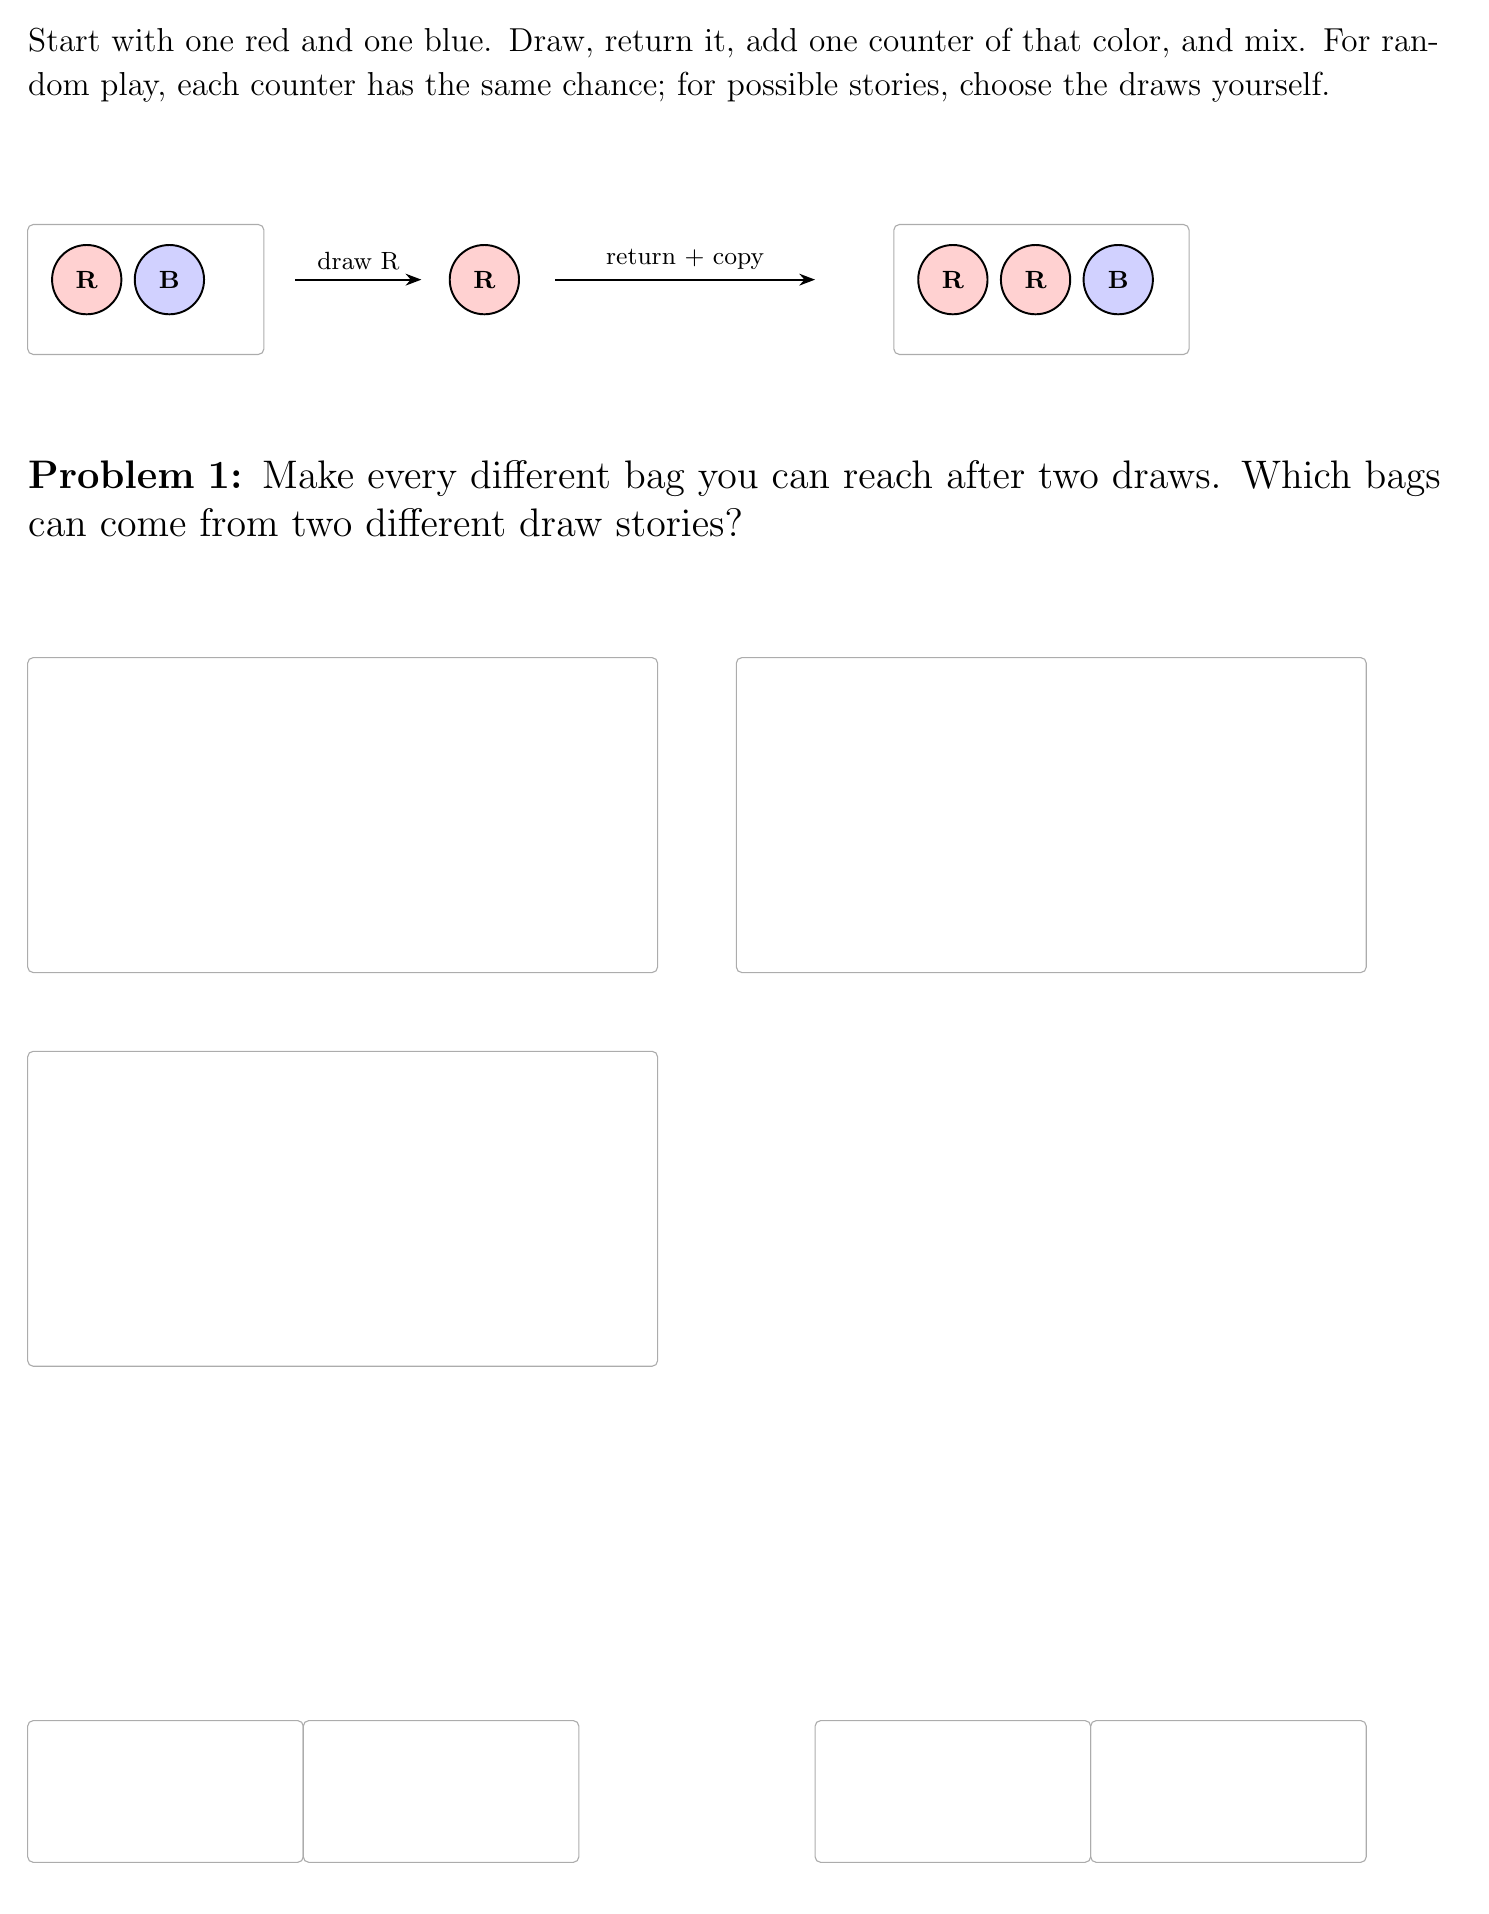
\begin{tikzpicture}[x=1cm,y=1cm]\path[use as bounding box] (0,0) rectangle (18.2,-23.6);
\node[anchor=north west,text width=18cm,inner sep=0pt,font=\fontsize{13}{16}\selectfont] at (0,0) {Start with one red and one blue. Draw, return it, add one counter of that color, and mix. For random play, each counter has the same chance; for possible stories, choose the draws yourself.};
\draw[gray!65,rounded corners=2pt] (0,-2.5) rectangle (3,-4.15);
\draw[fill=red!18,line width=.7pt] (0.75,-3.2) circle (0.44);
\node[font=\bfseries\small] at (0.75,-3.2) {R};
\draw[fill=blue!18,line width=.7pt] (1.8,-3.2) circle (0.44);
\node[font=\bfseries\small] at (1.8,-3.2) {B};
\draw[-{Stealth[length=2mm]},line width=.8pt] (3.4,-3.2) -- (5,-3.2) node[midway,above,font=\small] {draw R};
\draw[fill=red!18,line width=.7pt] (5.8,-3.2) circle (0.44);
\node[font=\bfseries\small] at (5.8,-3.2) {R};
\draw[-{Stealth[length=2mm]},line width=.8pt] (6.7,-3.2) -- (10,-3.2) node[midway,above,font=\small] {return + copy};
\draw[gray!65,rounded corners=2pt] (11,-2.5) rectangle (14.75,-4.15);
\draw[fill=red!18,line width=.7pt] (11.75,-3.2) circle (0.44);
\node[font=\bfseries\small] at (11.75,-3.2) {R};
\draw[fill=red!18,line width=.7pt] (12.8,-3.2) circle (0.44);
\node[font=\bfseries\small] at (12.8,-3.2) {R};
\draw[fill=blue!18,line width=.7pt] (13.85,-3.2) circle (0.44);
\node[font=\bfseries\small] at (13.85,-3.2) {B};
\node[anchor=north west,text width=18cm,inner sep=0pt,font=\fontsize{14}{17}\selectfont] at (0,-5.5) {\textbf{Problem 1:} Make every different bag you can reach after two draws. Which bags can come from two different draw stories?};
\draw[gray!65,rounded corners=2pt] (0,-8) rectangle (8,-12);
\draw[gray!65,rounded corners=2pt] (9,-8) rectangle (17,-12);
\draw[gray!65,rounded corners=2pt] (0,-13) rectangle (8,-17);
\draw[gray!65,rounded corners=2pt] (0.0,-21.5) rectangle (3.5,-23.3);
\draw[gray!65,rounded corners=2pt] (3.5,-21.5) rectangle (7.0,-23.3);
\draw[gray!65,rounded corners=2pt] (10.0,-21.5) rectangle (13.5,-23.3);
\draw[gray!65,rounded corners=2pt] (13.5,-21.5) rectangle (17.0,-23.3);
\end{tikzpicture}
\newpage
\noindent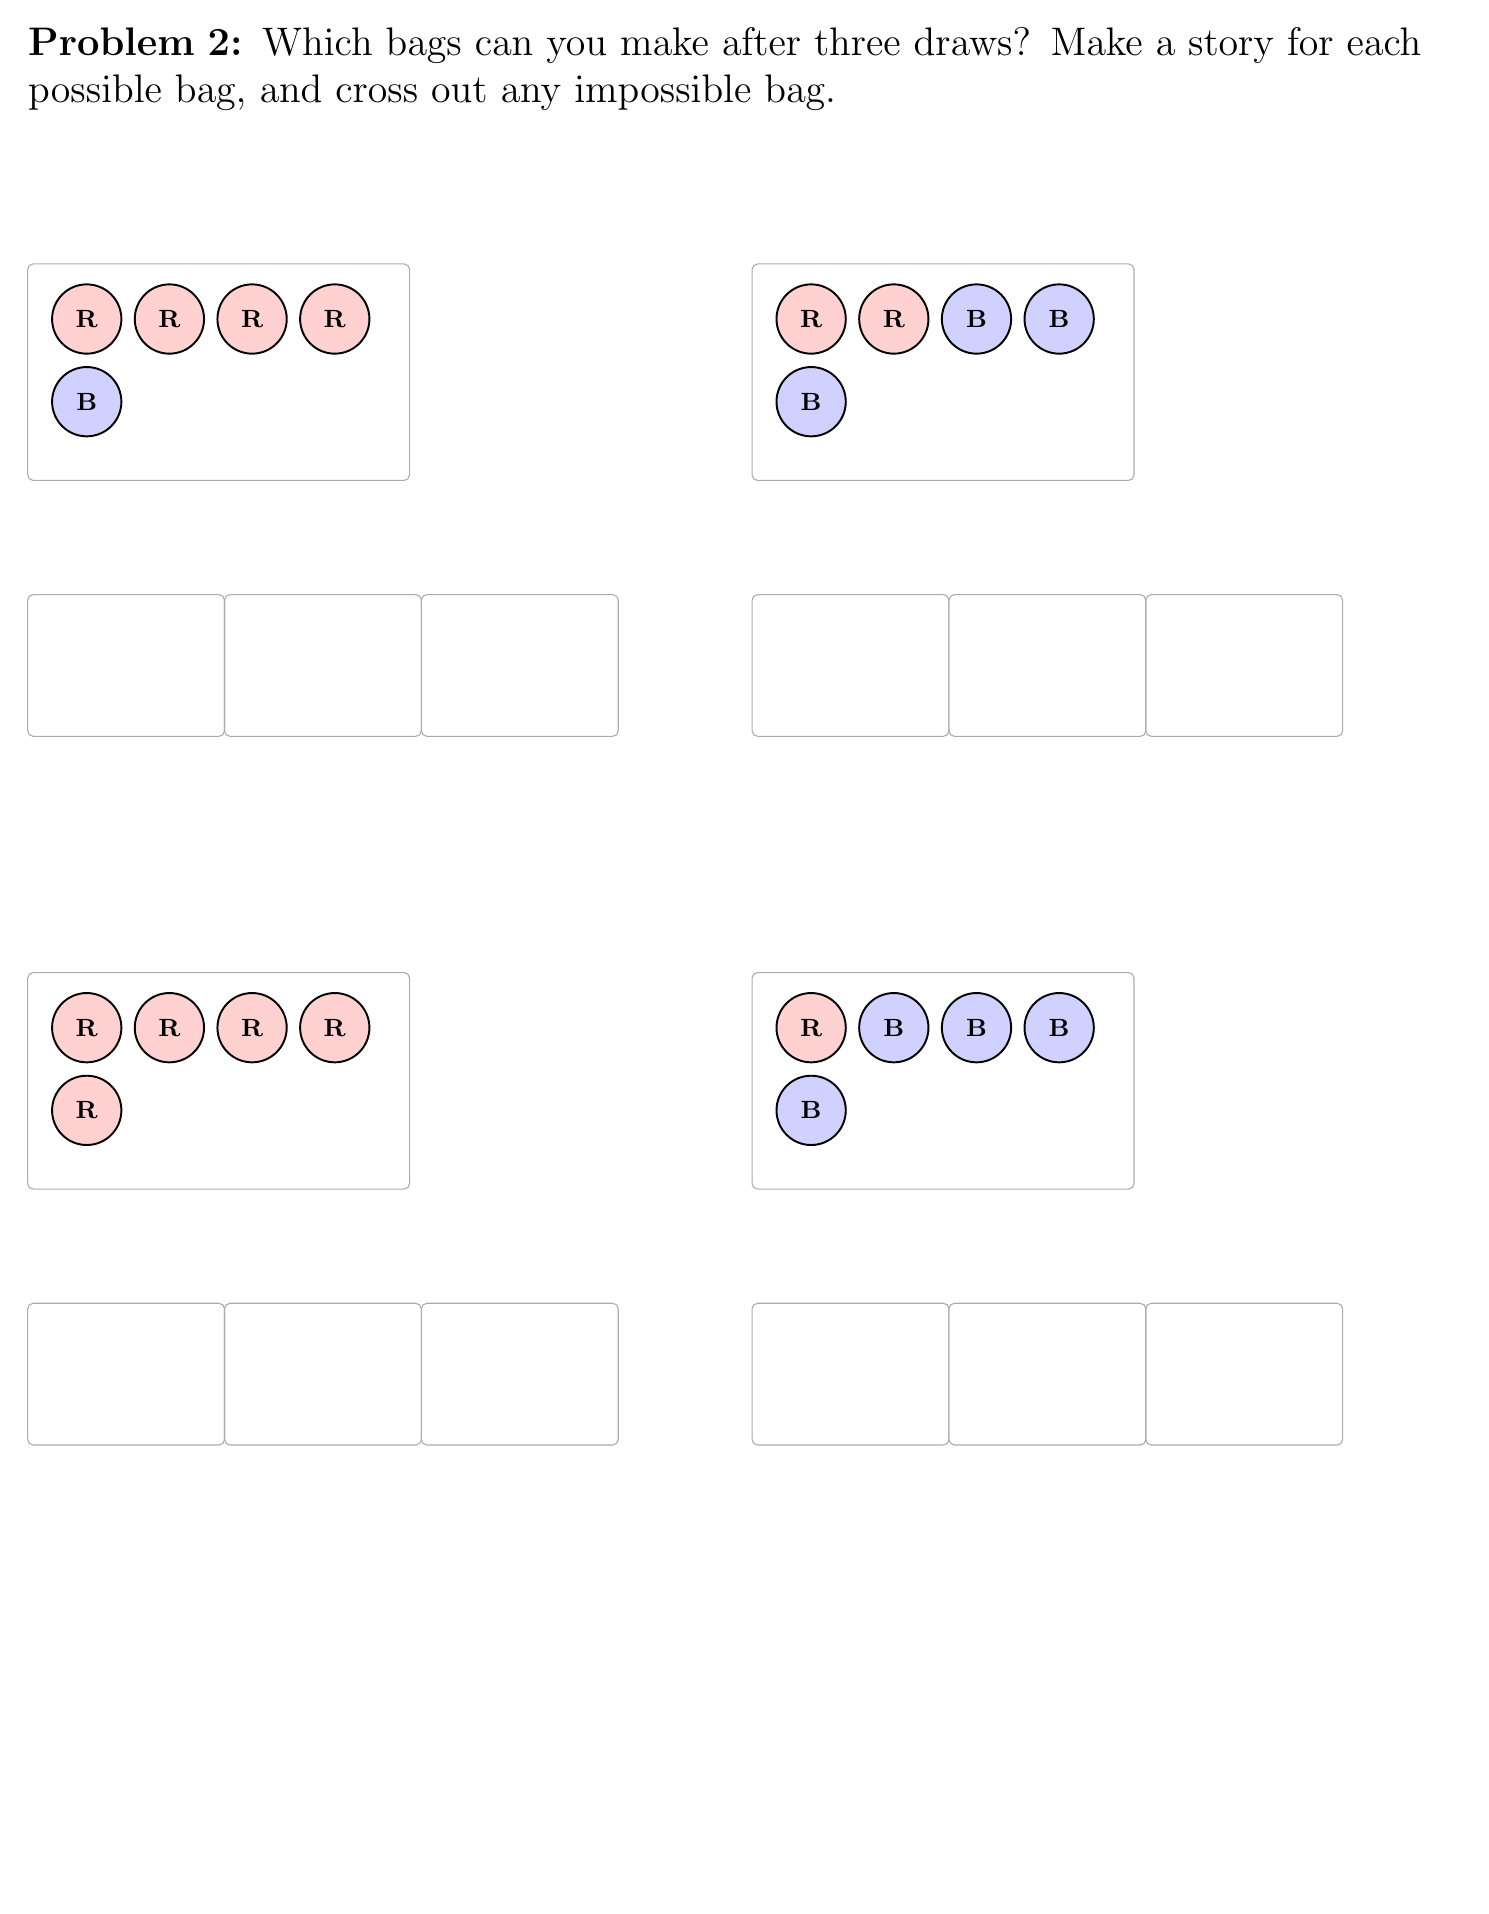
\begin{tikzpicture}[x=1cm,y=1cm]\path[use as bounding box] (0,0) rectangle (18.2,-23.6);
\node[anchor=north west,text width=18cm,inner sep=0pt,font=\fontsize{14}{17}\selectfont] at (0,0) {\textbf{Problem 2:} Which bags can you make after three draws? Make a story for each possible bag, and cross out any impossible bag.};
\draw[gray!65,rounded corners=2pt] (0.0,-3) rectangle (4.8500000000000005,-5.75);
\draw[fill=red!18,line width=.7pt] (0.75,-3.7) circle (0.44);
\node[font=\bfseries\small] at (0.75,-3.7) {R};
\draw[fill=red!18,line width=.7pt] (1.8,-3.7) circle (0.44);
\node[font=\bfseries\small] at (1.8,-3.7) {R};
\draw[fill=red!18,line width=.7pt] (2.85,-3.7) circle (0.44);
\node[font=\bfseries\small] at (2.85,-3.7) {R};
\draw[fill=red!18,line width=.7pt] (3.9000000000000004,-3.7) circle (0.44);
\node[font=\bfseries\small] at (3.9000000000000004,-3.7) {R};
\draw[fill=blue!18,line width=.7pt] (0.75,-4.75) circle (0.44);
\node[font=\bfseries\small] at (0.75,-4.75) {B};
\draw[gray!65,rounded corners=2pt] (0.0,-7.2) rectangle (2.5,-9.0);
\draw[gray!65,rounded corners=2pt] (2.5,-7.2) rectangle (5.0,-9.0);
\draw[gray!65,rounded corners=2pt] (5.0,-7.2) rectangle (7.5,-9.0);
\draw[gray!65,rounded corners=2pt] (9.2,-3) rectangle (14.05,-5.75);
\draw[fill=red!18,line width=.7pt] (9.95,-3.7) circle (0.44);
\node[font=\bfseries\small] at (9.95,-3.7) {R};
\draw[fill=red!18,line width=.7pt] (11.0,-3.7) circle (0.44);
\node[font=\bfseries\small] at (11.0,-3.7) {R};
\draw[fill=blue!18,line width=.7pt] (12.049999999999999,-3.7) circle (0.44);
\node[font=\bfseries\small] at (12.049999999999999,-3.7) {B};
\draw[fill=blue!18,line width=.7pt] (13.1,-3.7) circle (0.44);
\node[font=\bfseries\small] at (13.1,-3.7) {B};
\draw[fill=blue!18,line width=.7pt] (9.95,-4.75) circle (0.44);
\node[font=\bfseries\small] at (9.95,-4.75) {B};
\draw[gray!65,rounded corners=2pt] (9.2,-7.2) rectangle (11.7,-9.0);
\draw[gray!65,rounded corners=2pt] (11.7,-7.2) rectangle (14.2,-9.0);
\draw[gray!65,rounded corners=2pt] (14.2,-7.2) rectangle (16.7,-9.0);
\draw[gray!65,rounded corners=2pt] (0.0,-12) rectangle (4.8500000000000005,-14.75);
\draw[fill=red!18,line width=.7pt] (0.75,-12.7) circle (0.44);
\node[font=\bfseries\small] at (0.75,-12.7) {R};
\draw[fill=red!18,line width=.7pt] (1.8,-12.7) circle (0.44);
\node[font=\bfseries\small] at (1.8,-12.7) {R};
\draw[fill=red!18,line width=.7pt] (2.85,-12.7) circle (0.44);
\node[font=\bfseries\small] at (2.85,-12.7) {R};
\draw[fill=red!18,line width=.7pt] (3.9000000000000004,-12.7) circle (0.44);
\node[font=\bfseries\small] at (3.9000000000000004,-12.7) {R};
\draw[fill=red!18,line width=.7pt] (0.75,-13.75) circle (0.44);
\node[font=\bfseries\small] at (0.75,-13.75) {R};
\draw[gray!65,rounded corners=2pt] (0.0,-16.2) rectangle (2.5,-18.0);
\draw[gray!65,rounded corners=2pt] (2.5,-16.2) rectangle (5.0,-18.0);
\draw[gray!65,rounded corners=2pt] (5.0,-16.2) rectangle (7.5,-18.0);
\draw[gray!65,rounded corners=2pt] (9.2,-12) rectangle (14.05,-14.75);
\draw[fill=red!18,line width=.7pt] (9.95,-12.7) circle (0.44);
\node[font=\bfseries\small] at (9.95,-12.7) {R};
\draw[fill=blue!18,line width=.7pt] (11.0,-12.7) circle (0.44);
\node[font=\bfseries\small] at (11.0,-12.7) {B};
\draw[fill=blue!18,line width=.7pt] (12.049999999999999,-12.7) circle (0.44);
\node[font=\bfseries\small] at (12.049999999999999,-12.7) {B};
\draw[fill=blue!18,line width=.7pt] (13.1,-12.7) circle (0.44);
\node[font=\bfseries\small] at (13.1,-12.7) {B};
\draw[fill=blue!18,line width=.7pt] (9.95,-13.75) circle (0.44);
\node[font=\bfseries\small] at (9.95,-13.75) {B};
\draw[gray!65,rounded corners=2pt] (9.2,-16.2) rectangle (11.7,-18.0);
\draw[gray!65,rounded corners=2pt] (11.7,-16.2) rectangle (14.2,-18.0);
\draw[gray!65,rounded corners=2pt] (14.2,-16.2) rectangle (16.7,-18.0);
\end{tikzpicture}
\newpage
\noindent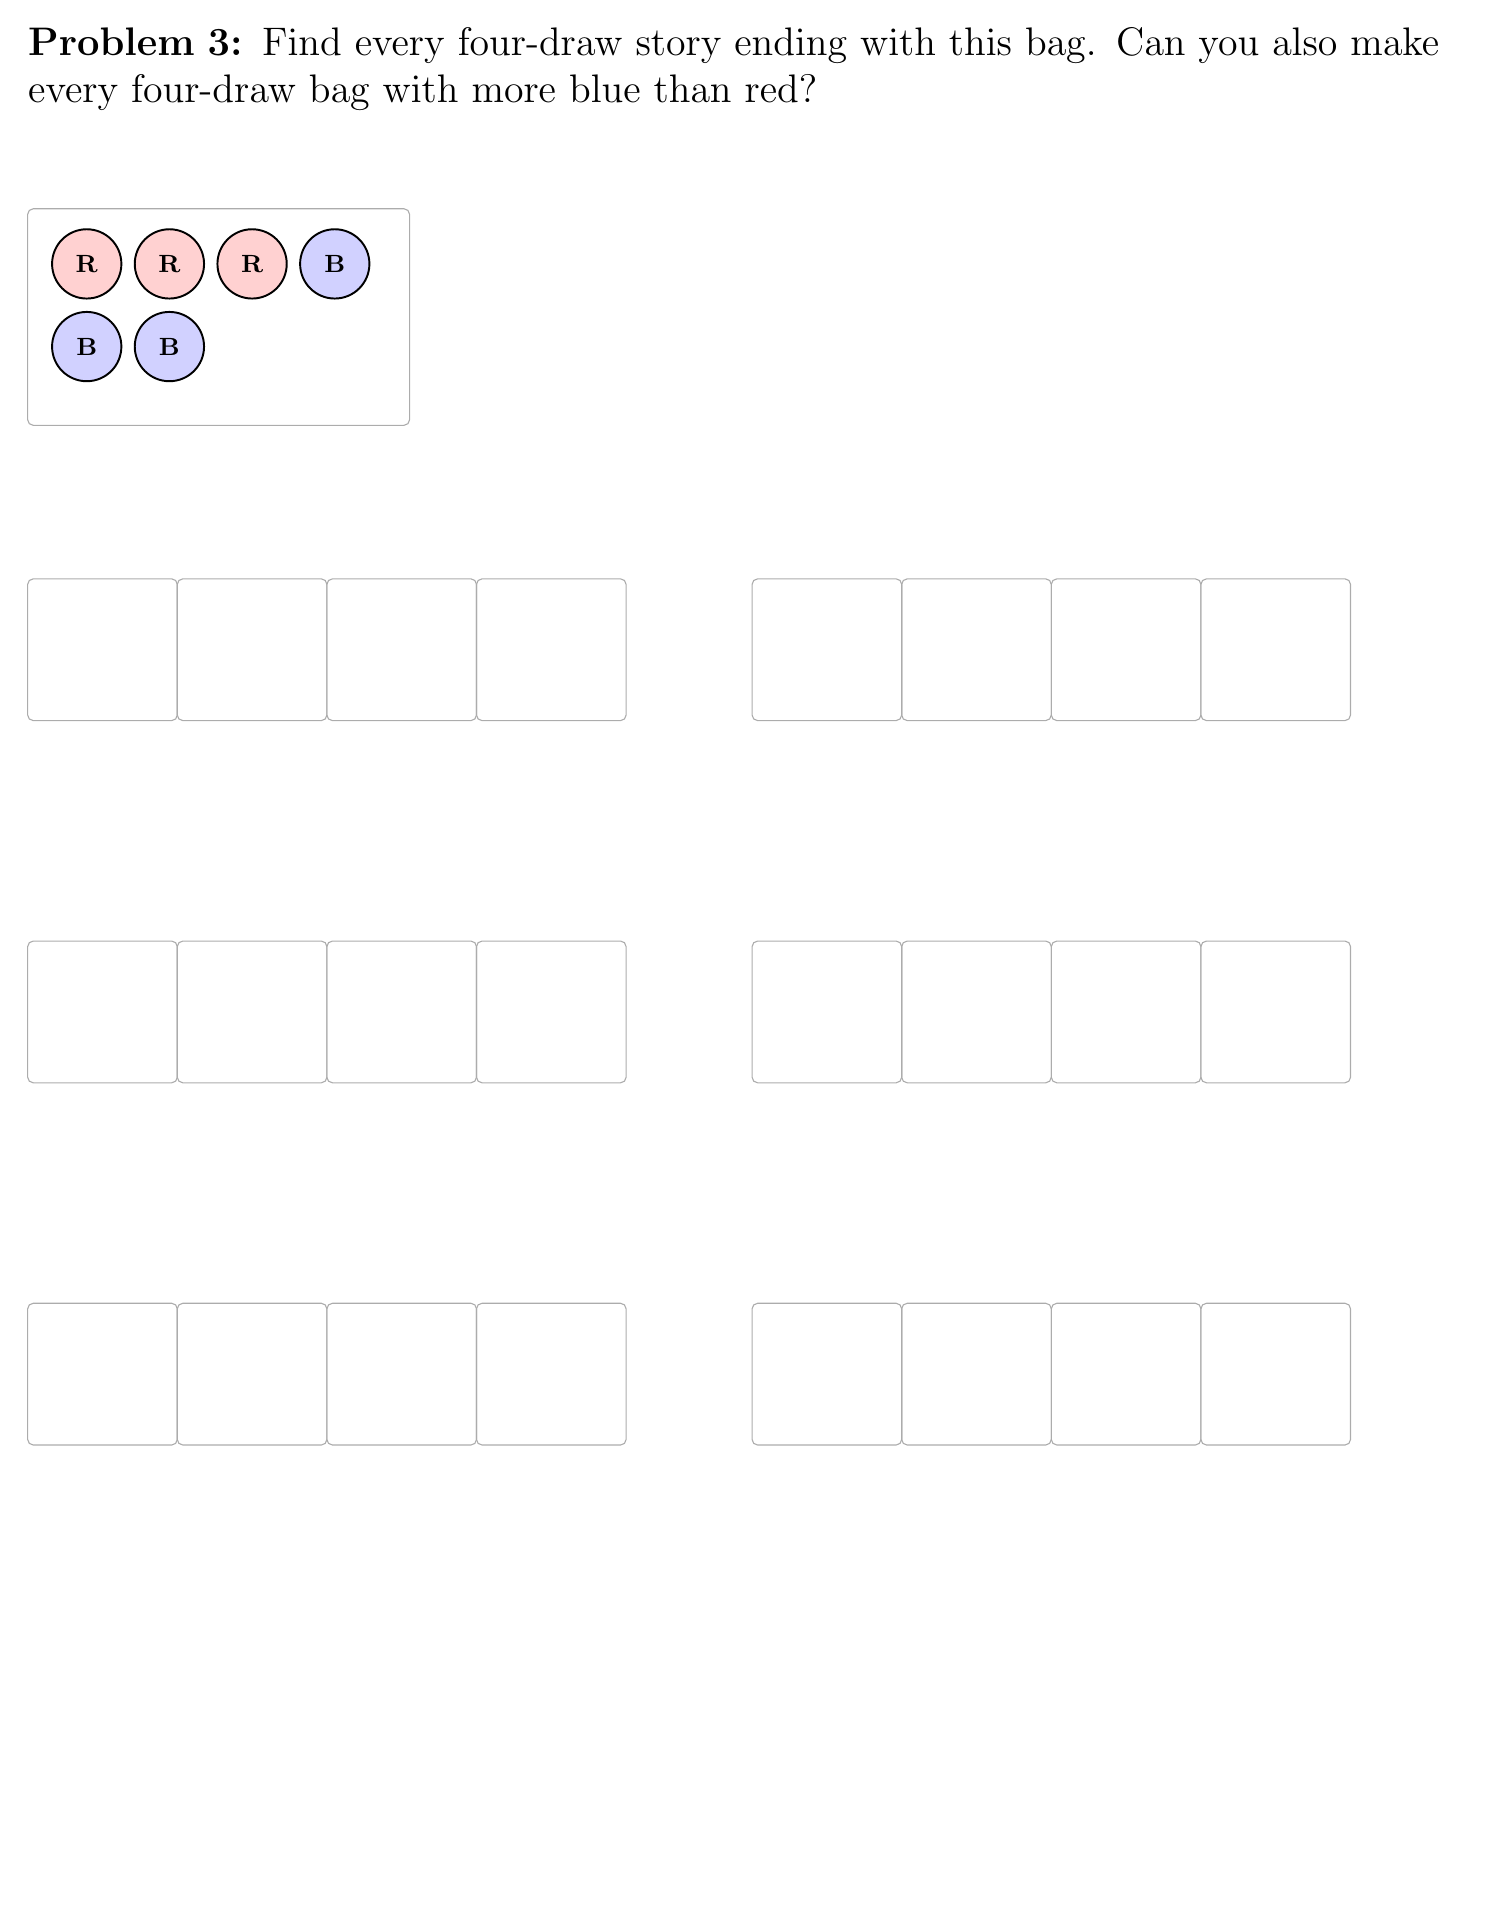
\begin{tikzpicture}[x=1cm,y=1cm]\path[use as bounding box] (0,0) rectangle (18.2,-23.6);
\node[anchor=north west,text width=18cm,inner sep=0pt,font=\fontsize{14}{17}\selectfont] at (0,0) {\textbf{Problem 3:} Find every four-draw story ending with this bag. Can you also make every four-draw bag with more blue than red?};
\draw[gray!65,rounded corners=2pt] (0,-2.3) rectangle (4.8500000000000005,-5.05);
\draw[fill=red!18,line width=.7pt] (0.75,-3.0) circle (0.44);
\node[font=\bfseries\small] at (0.75,-3.0) {R};
\draw[fill=red!18,line width=.7pt] (1.8,-3.0) circle (0.44);
\node[font=\bfseries\small] at (1.8,-3.0) {R};
\draw[fill=red!18,line width=.7pt] (2.85,-3.0) circle (0.44);
\node[font=\bfseries\small] at (2.85,-3.0) {R};
\draw[fill=blue!18,line width=.7pt] (3.9000000000000004,-3.0) circle (0.44);
\node[font=\bfseries\small] at (3.9000000000000004,-3.0) {B};
\draw[fill=blue!18,line width=.7pt] (0.75,-4.05) circle (0.44);
\node[font=\bfseries\small] at (0.75,-4.05) {B};
\draw[fill=blue!18,line width=.7pt] (1.8,-4.05) circle (0.44);
\node[font=\bfseries\small] at (1.8,-4.05) {B};
\draw[gray!65,rounded corners=2pt] (0.0,-7.0) rectangle (1.9,-8.8);
\draw[gray!65,rounded corners=2pt] (1.9,-7.0) rectangle (3.8,-8.8);
\draw[gray!65,rounded corners=2pt] (3.8,-7.0) rectangle (5.699999999999999,-8.8);
\draw[gray!65,rounded corners=2pt] (5.699999999999999,-7.0) rectangle (7.6,-8.8);
\draw[gray!65,rounded corners=2pt] (9.2,-7.0) rectangle (11.1,-8.8);
\draw[gray!65,rounded corners=2pt] (11.1,-7.0) rectangle (13.0,-8.8);
\draw[gray!65,rounded corners=2pt] (13.0,-7.0) rectangle (14.9,-8.8);
\draw[gray!65,rounded corners=2pt] (14.899999999999999,-7.0) rectangle (16.799999999999997,-8.8);
\draw[gray!65,rounded corners=2pt] (0.0,-11.6) rectangle (1.9,-13.4);
\draw[gray!65,rounded corners=2pt] (1.9,-11.6) rectangle (3.8,-13.4);
\draw[gray!65,rounded corners=2pt] (3.8,-11.6) rectangle (5.699999999999999,-13.4);
\draw[gray!65,rounded corners=2pt] (5.699999999999999,-11.6) rectangle (7.6,-13.4);
\draw[gray!65,rounded corners=2pt] (9.2,-11.6) rectangle (11.1,-13.4);
\draw[gray!65,rounded corners=2pt] (11.1,-11.6) rectangle (13.0,-13.4);
\draw[gray!65,rounded corners=2pt] (13.0,-11.6) rectangle (14.9,-13.4);
\draw[gray!65,rounded corners=2pt] (14.899999999999999,-11.6) rectangle (16.799999999999997,-13.4);
\draw[gray!65,rounded corners=2pt] (0.0,-16.2) rectangle (1.9,-18.0);
\draw[gray!65,rounded corners=2pt] (1.9,-16.2) rectangle (3.8,-18.0);
\draw[gray!65,rounded corners=2pt] (3.8,-16.2) rectangle (5.699999999999999,-18.0);
\draw[gray!65,rounded corners=2pt] (5.699999999999999,-16.2) rectangle (7.6,-18.0);
\draw[gray!65,rounded corners=2pt] (9.2,-16.2) rectangle (11.1,-18.0);
\draw[gray!65,rounded corners=2pt] (11.1,-16.2) rectangle (13.0,-18.0);
\draw[gray!65,rounded corners=2pt] (13.0,-16.2) rectangle (14.9,-18.0);
\draw[gray!65,rounded corners=2pt] (14.899999999999999,-16.2) rectangle (16.799999999999997,-18.0);
\end{tikzpicture}
\newpage
\noindent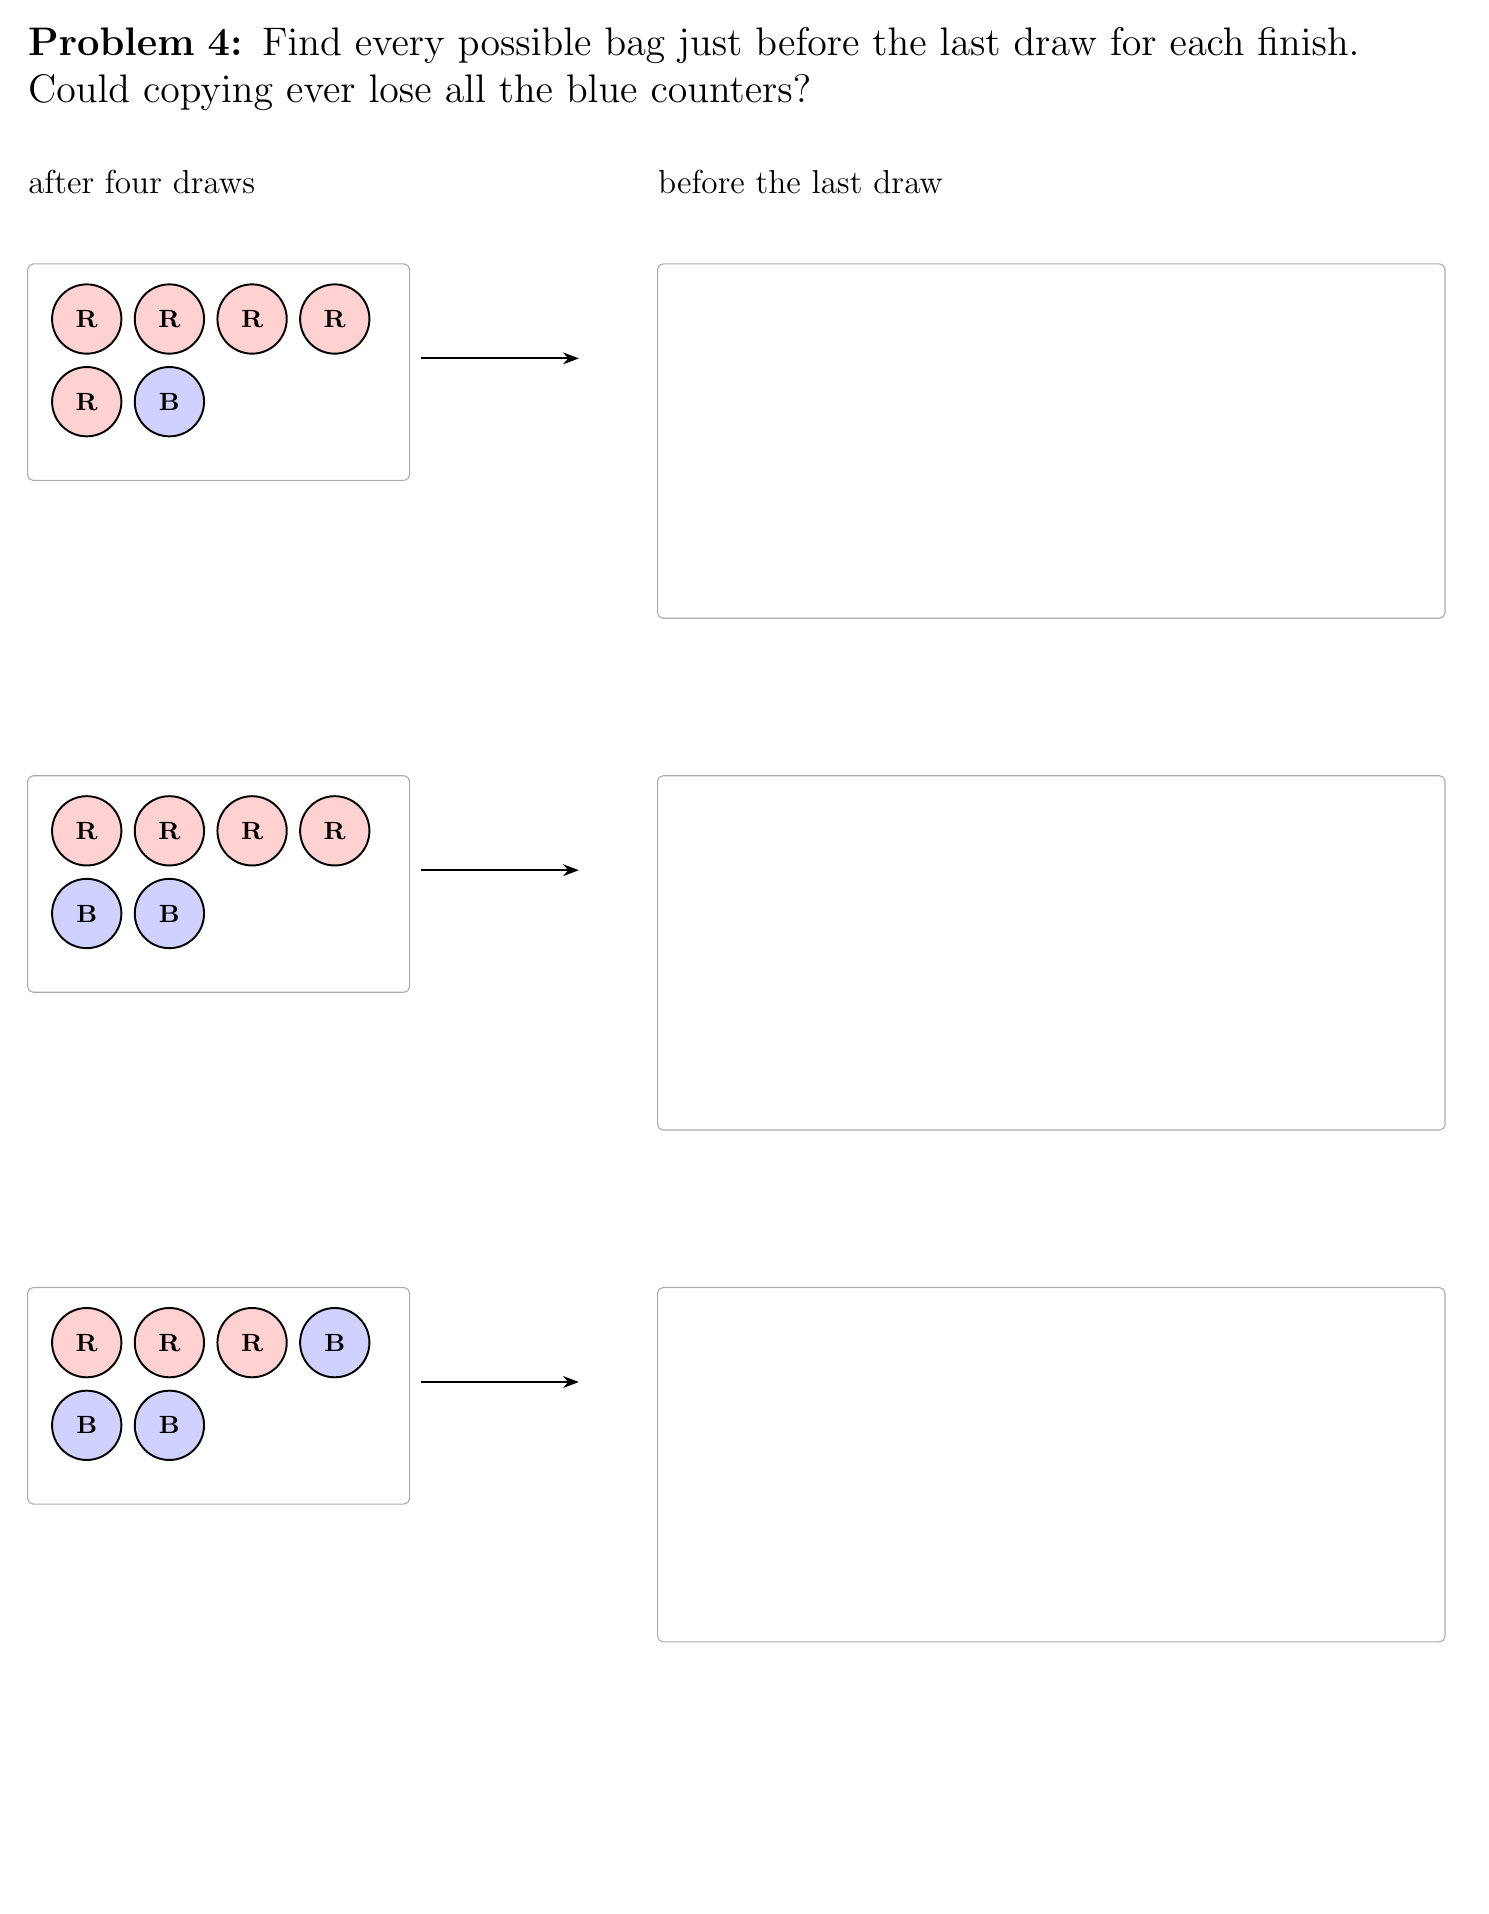
\begin{tikzpicture}[x=1cm,y=1cm]\path[use as bounding box] (0,0) rectangle (18.2,-23.6);
\node[anchor=north west,text width=18cm,inner sep=0pt,font=\fontsize{14}{17}\selectfont] at (0,0) {\textbf{Problem 4:} Find every possible bag just before the last draw for each finish. Could copying ever lose all the blue counters?};
\node[anchor=north west,text width=6cm,inner sep=0pt,font=\fontsize{12}{15}\selectfont] at (0,-1.8) {after four draws};
\node[anchor=north west,text width=10cm,inner sep=0pt,font=\fontsize{12}{15}\selectfont] at (8,-1.8) {before the last draw};
\draw[gray!65,rounded corners=2pt] (0,-3.0) rectangle (4.8500000000000005,-5.75);
\draw[fill=red!18,line width=.7pt] (0.75,-3.7) circle (0.44);
\node[font=\bfseries\small] at (0.75,-3.7) {R};
\draw[fill=red!18,line width=.7pt] (1.8,-3.7) circle (0.44);
\node[font=\bfseries\small] at (1.8,-3.7) {R};
\draw[fill=red!18,line width=.7pt] (2.85,-3.7) circle (0.44);
\node[font=\bfseries\small] at (2.85,-3.7) {R};
\draw[fill=red!18,line width=.7pt] (3.9000000000000004,-3.7) circle (0.44);
\node[font=\bfseries\small] at (3.9000000000000004,-3.7) {R};
\draw[fill=red!18,line width=.7pt] (0.75,-4.75) circle (0.44);
\node[font=\bfseries\small] at (0.75,-4.75) {R};
\draw[fill=blue!18,line width=.7pt] (1.8,-4.75) circle (0.44);
\node[font=\bfseries\small] at (1.8,-4.75) {B};
\draw[-{Stealth[length=2mm]},line width=.8pt] (5,-4.2) -- (7,-4.2) node[midway,above,font=\small] {};
\draw[gray!65,rounded corners=2pt] (8,-3.0) rectangle (18,-7.5);
\draw[gray!65,rounded corners=2pt] (0,-9.5) rectangle (4.8500000000000005,-12.25);
\draw[fill=red!18,line width=.7pt] (0.75,-10.2) circle (0.44);
\node[font=\bfseries\small] at (0.75,-10.2) {R};
\draw[fill=red!18,line width=.7pt] (1.8,-10.2) circle (0.44);
\node[font=\bfseries\small] at (1.8,-10.2) {R};
\draw[fill=red!18,line width=.7pt] (2.85,-10.2) circle (0.44);
\node[font=\bfseries\small] at (2.85,-10.2) {R};
\draw[fill=red!18,line width=.7pt] (3.9000000000000004,-10.2) circle (0.44);
\node[font=\bfseries\small] at (3.9000000000000004,-10.2) {R};
\draw[fill=blue!18,line width=.7pt] (0.75,-11.25) circle (0.44);
\node[font=\bfseries\small] at (0.75,-11.25) {B};
\draw[fill=blue!18,line width=.7pt] (1.8,-11.25) circle (0.44);
\node[font=\bfseries\small] at (1.8,-11.25) {B};
\draw[-{Stealth[length=2mm]},line width=.8pt] (5,-10.7) -- (7,-10.7) node[midway,above,font=\small] {};
\draw[gray!65,rounded corners=2pt] (8,-9.5) rectangle (18,-14.0);
\draw[gray!65,rounded corners=2pt] (0,-16.0) rectangle (4.8500000000000005,-18.75);
\draw[fill=red!18,line width=.7pt] (0.75,-16.7) circle (0.44);
\node[font=\bfseries\small] at (0.75,-16.7) {R};
\draw[fill=red!18,line width=.7pt] (1.8,-16.7) circle (0.44);
\node[font=\bfseries\small] at (1.8,-16.7) {R};
\draw[fill=red!18,line width=.7pt] (2.85,-16.7) circle (0.44);
\node[font=\bfseries\small] at (2.85,-16.7) {R};
\draw[fill=blue!18,line width=.7pt] (3.9000000000000004,-16.7) circle (0.44);
\node[font=\bfseries\small] at (3.9000000000000004,-16.7) {B};
\draw[fill=blue!18,line width=.7pt] (0.75,-17.75) circle (0.44);
\node[font=\bfseries\small] at (0.75,-17.75) {B};
\draw[fill=blue!18,line width=.7pt] (1.8,-17.75) circle (0.44);
\node[font=\bfseries\small] at (1.8,-17.75) {B};
\draw[-{Stealth[length=2mm]},line width=.8pt] (5,-17.2) -- (7,-17.2) node[midway,above,font=\small] {};
\draw[gray!65,rounded corners=2pt] (8,-16.0) rectangle (18,-20.5);
\end{tikzpicture}
\end{document}
